
%%%%%%%%%%%%%%%%%%%%%%%%%%%%%%%%%%%%%%%%%
% Programming/Coding Assignment
% LaTeX Template
%
% This template has been downloaded from:
% http://www.latextemplates.com
%
% Original author:
% Ted Pavlic (http://www.tedpavlic.com)
%
% Note:
% The \lipsum[#] commands throughout this template generate dummy text
% to fill the template out. These commands should all be removed when 
% writing assignment content.
%
% This template uses a Perl script as an example snippet of code, most other
% languages are also usable. Configure them in the "CODE INCLUSION 
% CONFIGURATION" section.
%
%%%%%%%%%%%%%%%%%%%%%%%%%%%%%%%%%%%%%%%%%

%----------------------------------------------------------------------------------------
%	PACKAGES AND OTHER DOCUMENT CONFIGURATIONS
%----------------------------------------------------------------------------------------



\documentclass{article}

\usepackage{fancyhdr} % Required for custom headers
\usepackage{lastpage} % Required to determine the last page for the footer
\usepackage{extramarks} % Required for headers and footers
\usepackage[usenames,dvipsnames]{color} % Required for custom colors
\usepackage{graphicx} % Required to insert images
\usepackage{listings} % Required for insertion of code
\usepackage{courier} % Required for the courier font
\usepackage{lipsum} % Used for inserting dummy 'Lorem ipsum' text into the template
\usepackage{setspace}
\usepackage{color}
\usepackage{comment}
\usepackage{caption}

\usepackage{hyperref}
\usepackage{natbib}
\usepackage{underscore}
\usepackage{subfigure}
\usepackage{fixltx2e}

\hypersetup{
    colorlinks=true,
    linkcolor=blue,
    filecolor=magenta,      
    urlcolor=cyan,
    breaklinks=true
}

\usepackage[]{algorithm2e}
\usepackage{pdfpages}
\usepackage{tikz}




%For python inclusion (http://widerin.org/blog/syntax-highlighting-for-python-scripts-in-latex-documents)
\definecolor{Code}{rgb}{0,0,0}
\definecolor{Decorators}{rgb}{0.5,0.5,0.5}
\definecolor{Numbers}{rgb}{0.5,0,0}
\definecolor{MatchingBrackets}{rgb}{0.25,0.5,0.5}
\definecolor{Keywords}{rgb}{0,0,1}
\definecolor{self}{rgb}{0,0,0}
\definecolor{Strings}{rgb}{0,0.63,0}
\definecolor{Comments}{rgb}{0,0.63,1}
\definecolor{Backquotes}{rgb}{0,0,0}
\definecolor{Classname}{rgb}{0,0,0}
\definecolor{FunctionName}{rgb}{0,0,0}
\definecolor{Operators}{rgb}{0,0,0}
\definecolor{Background}{rgb}{0.98,0.98,0.98}

% Margins
\topmargin=-0.45in
\evensidemargin=0in
\oddsidemargin=0in
\textwidth=6.5in
\textheight=9.0in
\headsep=0.25in

\linespread{1.1} % Line spacing

% Set up the header and footer
\pagestyle{fancy}
\lhead{\hmwkAuthorName} % Top left header
\chead{\hmwkClass\ (\hmwkClassInstructor\ \hmwkClassTime): \hmwkTitle} % Top center head
\chead{\hmwkClass\ (\hmwkClassInstructor): \hmwkTitle} % Top center head
\rhead{\firstxmark} % Top right header
\lfoot{\lastxmark} % Bottom left footer
\cfoot{} % Bottom center footer
\rfoot{Page\ \thepage\ of\ \protect\pageref{LastPage}} % Bottom right footer
\renewcommand\headrulewidth{0.4pt} % Size of the header rule
\renewcommand\footrulewidth{0.4pt} % Size of the footer rule

\setlength\parindent{0pt} % Removes all indentation from paragraphs

%----------------------------------------------------------------------------------------
%	CODE INCLUSION CONFIGURATION
%----------------------------------------------------------------------------------------

\definecolor{MyDarkGreen}{rgb}{0.0,0.4,0.0} % This is the color used for comments
\lstloadlanguages{Perl} % Load Perl syntax for listings, for a list of other languages supported see: ftp://ftp.tex.ac.uk/tex-archive/macros/latex/contrib/listings/listings.pdf
\lstset{language=Perl, % Use Perl in this example
        frame=single, % Single frame around code
        basicstyle=\small\ttfamily, % Use small true type font
        keywordstyle=[1]\color{Blue}\bf, % Perl functions bold and blue
        keywordstyle=[2]\color{Purple}, % Perl function arguments purple
        keywordstyle=[3]\color{Blue}\underbar, % Custom functions underlined and blue
        identifierstyle=, % Nothing special about identifiers                                         
        commentstyle=\usefont{T1}{pcr}{m}{sl}\color{MyDarkGreen}\small, % Comments small dark green courier font
        stringstyle=\color{Purple}, % Strings are purple
        showstringspaces=false, % Don't put marks in string spaces
        tabsize=5, % 5 spaces per tab
        %
        % Put standard Perl functions not included in the default language here
        morekeywords={rand},
        %
        % Put Perl function parameters here
        morekeywords=[2]{on, off, interp},
        %
        % Put user defined functions here
        morekeywords=[3]{test},
       	%
        morecomment=[l][\color{Blue}]{...}, % Line continuation (...) like blue comment
        numbers=left, % Line numbers on left
        firstnumber=1, % Line numbers start with line 1
        numberstyle=\tiny\color{Blue}, % Line numbers are blue and small
        stepnumber=5 % Line numbers go in steps of 5
}

% Creates a new command to include a perl script, the first parameter is the filename of the script (without .pl), the second parameter is the caption
\newcommand{\perlscript}[2]{
\begin{itemize}
\item[]\lstinputlisting[caption=#2,label=#1]{#1.pl}
\end{itemize}
}


%----------------------------------------------------------------------------------------
%	DOCUMENT STRUCTURE COMMANDS
%	Skip this unless you know what you're doing
%----------------------------------------------------------------------------------------

% Header and footer for when a page split occurs within a problem environment
\newcommand{\enterProblemHeader}[1]{
\nobreak\extramarks{#1}{#1 continued on next page\ldots}\nobreak
\nobreak\extramarks{#1 (continued)}{#1 continued on next page\ldots}\nobreak
}

% Header and footer for when a page split occurs between problem environments
\newcommand{\exitProblemHeader}[1]{
\nobreak\extramarks{#1 (continued)}{#1 continued on next page\ldots}\nobreak
\nobreak\extramarks{#1}{}\nobreak
}

\setcounter{secnumdepth}{0} % Removes default section numbers
\newcounter{homeworkProblemCounter} % Creates a counter to keep track of the number of problems

\newcommand{\homeworkProblemName}{}
\newenvironment{homeworkProblem}[1][Problem \arabic{homeworkProblemCounter}]{ % Makes a new environment called homeworkProblem which takes 1 argument (custom name) but the default is "Problem #"
\stepcounter{homeworkProblemCounter} % Increase counter for number of problems
\renewcommand{\homeworkProblemName}{#1} % Assign \homeworkProblemName the name of the problem
\section{\homeworkProblemName} % Make a section in the document with the custom problem count
\enterProblemHeader{\homeworkProblemName} % Header and footer within the environment
}{
\exitProblemHeader{\homeworkProblemName} % Header and footer after the environment
}

\newcommand{\problemAnswer}[1]{ % Defines the problem answer command with the content as the only argument
\noindent\framebox[\columnwidth][c]{\begin{minipage}{0.98\columnwidth}#1\end{minipage}} % Makes the box around the problem answer and puts the content inside
}

\newcommand{\homeworkSectionName}{}
\newenvironment{homeworkSection}[1]{ % New environment for sections within homework problems, takes 1 argument - the name of the section
\renewcommand{\homeworkSectionName}{#1} % Assign \homeworkSectionName to the name of the section from the environment argument
\subsection{\homeworkSectionName} % Make a subsection with the custom name of the subsection
\enterProblemHeader{\homeworkProblemName\ [\homeworkSectionName]} % Header and footer within the environment
}{
\enterProblemHeader{\homeworkProblemName} % Header and footer after the environment
}

%----------------------------------------------------------------------------------------
%	NAME AND CLASS SECTION
%----------------------------------------------------------------------------------------

\newcommand{\hmwkTitle}{Assignment\ \#1 } % Assignment title
%\newcommand{\hmwkDueDate}{Monday,\ January\ 1,\ 2012} % Due date
\newcommand{\hmwkClass}{Web Science} % Course/class
%\newcommand{\hmwkClassTime}{10:30am} % Class/lecture time
\newcommand{\hmwkClassInstructor}{Alexander Nwala} % Teacher/lecturer
\newcommand{\hmwkAuthorName}{Puneeth Bikkasandra} % Your name

%----------------------------------------------------------------------------------------
%	TITLE PAGE
%----------------------------------------------------------------------------------------

\title{
\vspace{2in}
\textmd{\textbf{\hmwkClass:\ \hmwkTitle}}\\
%\normalsize\vspace{0.1in}\small{Due\ on\ \hmwkDueDate}\\
%\vspace{0.1in}\large{\textit{\hmwkClassInstructor\ \hmwkClassTime}}
\vspace{0.1in}\large{\textit{\hmwkClassInstructor}}
\vspace{3in}
}

\author{\textbf{\hmwkAuthorName}}
\date{Sunday, January 28, 2018} % Insert date here if you want it to appear below your name

%----------------------------------------------------------------------------------------

\begin{document}

\maketitle
\newpage



%----------------------------------------------------------------------------------------
%	TABLE OF CONTENTS
%----------------------------------------------------------------------------------------

%\setcounter{tocdepth}{1} % Uncomment this line if you don't want subsections listed in the ToC

\newpage
\tableofcontents
\newpage

%----------------------------------------------------------------------------------------
%	PROBLEM 1
%----------------------------------------------------------------------------------------

% To have just one problem per page, simply put a \clearpage after each problem

\begin{homeworkProblem}

Demonstrate that you know how to use "curl" well enough to correctly POST data to a form.Show that the HTML response that is returned is "correct".That is, the server should take the arguments you POSTed and\\
build a response accordingly.  Save the HTML response to a file and then view that file in a browser and take a screen shot.\\

%\problemAnswer{
 \textbf{SOLUTION :}\\
  \begin{verbatim}
  curl -i -d "fname=Puneeth \& lname=Shankar" -X POST 
  http://www.cs.odu.edu/\~anwala/files/temp/namesEcho.php
  \end{verbatim}
  
\begin{figure}[h]
  \centering
    \includegraphics[width=0.5\textwidth]{webScience}
      \caption{Sample 'curl' with POST}
\end{figure}
 
%}

\end{homeworkProblem}
\clearpage
\newpage
%----------------------------------------------------------------------------------------
%   PROBLEM 2
%----------------------------------------------------------------------------------------

\begin{homeworkProblem}
 
Write a Python program that:\\
\begin{enumerate}
\item \textbf{} takes as a command line argument a web page
\item \textbf{} extracts all the links from the page
\item \textbf{} lists all the links that result in PDF files, and prints out the bytes for each of the links.  \\
			(note: be sure to follow all the redirects until the link terminates with a "200 OK".)
\item \textbf{} show that the program works on 3 different URIs, one of which needs to be:\\
		     \url{http://www.cs.odu.edu/~mln/teaching/cs532-s17/test/pdfs.html}\\
 \end{enumerate}
%\problemAnswer{
 \textbf{SOLUTION}\\\\
 The solution for this problem is outlined by the following steps:\\
 \begin{enumerate}
 \item \textbf{Command Line Arguments :} Programmatically referred as \textbf{sys.argv} contains a list of arguments, which could be passed to the program. The below command takes 3 web pages as the arguments.
 \begin{verbatim}
   python Assignment1.py http://www.google.com  https://www.facebook.com  
   	http://www.cs.odu.edu/~mln/teaching/cs532-s17/test/pdfs.html	
 \end{verbatim}
  \item \textbf{Extracting the Links from the Web Pages :} The below code in Listing 1; extracts the web links, captures the redirection and finally saves in an independent file.
 
 \begin{lstlisting}[language=Python, caption=Assignment1.py]
import requests
import sys
from BeautifulSoup import BeautifulSoup
links = []
def getURL(page):
    
    start_link = page.find("a href")
    if start_link == -1:
        return None, 0
    start_quote = page.find('"', start_link)
    end_quote = page.find('"', start_quote + 1)
    url = page[start_quote + 1: end_quote]
    return url, end_quote

def checkForRedirection(link1):
    response = requests.get(link1)
    if('Response [200]' in response):
        return link1
    else:
        return response.url
        
for webpage in sys.argv:
    baseUrl = webpage
    if(webpage == 'Assignment1.py'):
        continue
    else:
        response = requests.get(webpage)
        page = str(BeautifulSoup(response.content))
        while True:
            url, n = getURL(page)
            page = page[n:]
            if url:
                if('://' in url):
                    url = checkForRedirection(url)
                    links.append(url)
                else:
                    url = checkForRedirection(baseUrl + url)
                    links.append(url)
            else:
                break

pdf = open("pdfLinks.txt","w")
justLinks = open("justLinks.txt","w")
for link in links:
    response = requests.get(link)
    if(response.headers['content-type'] == 'application/pdf'):
        size = response.headers['content-Length']
        line = pdf.write(link+"      : Length - "+size+" bytes")
        line = pdf.write('\n')
        line = justLinks.write(link)
        line = justLinks.write('\n')
    else:
        line = justLinks.write(link)
        line = justLinks.write('\n')
pdf.close()
justLinks.close() 
\end{lstlisting}
%}
\textbf{Links obtained after extraction:}

\begin{lstlisting}[caption=Extracted Links]
http://www.google.com/history/optout?hl=en&nzb=1
https://www.google.com/preferences?hl=en
https://www.google.com/advanced_search?hl=en&amp;authuser=0
https://translate.google.com/
https://www.google.com/intl/en/ads/
https://www.google.com/services/
https://plus.google.com/116899029375914044550
https://www.google.com/intl/en/about/
https://www.google.com/intl/en/policies/privacy/
https://www.google.com/intl/en/policies/terms/
https://www.google.com/history%5C
https://twitter.com/webscidl
http://www.dlib.org/dlib/november15/vandesompel/11vandesompel.html
https://arxiv.org/abs/1508.02315
https://arxiv.org/abs/1508.02315
http://www.cs.odu.edu/~mln/pubs/ht-2015/hypertext-2015-temporal-violations.pdf
http://www.cs.odu.edu/~mln/pubs/tpdl-2015/tpdl-2015-annotations.pdf
https://arxiv.org/pdf/1512.06195.pdf
http://www.cs.odu.edu/~mln/pubs/tpdl-2015/tpdl-2015-off-topic.pdf
http://www.cs.odu.edu/~mln/pubs/tpdl-2015/tpdl-2015-stories.pdf
http://www.cs.odu.edu/~mln/pubs/tpdl-2015/tpdl-2015-profiling.pdf
https://link.springer.com/article/10.1007%2Fs00799-015-0150-6
http://www.cs.odu.edu/~mln/pubs/jcdl-2014/jcdl-2014-brunelle-damage.pdf
https://arxiv.org/abs/1506.06279
https://link.springer.com/article/10.1007%2Fs00799-015-0155-1
http://www.cs.odu.edu/~mln/pubs/jcdl-2015/jcdl-2015-temporal-intention.pdf
http://www.cs.odu.edu/~mln/pubs/jcdl-2015/jcdl-2015-mink.pdf
http://www.cs.odu.edu/~mln/pubs/jcdl-2015/jcdl-2015-arabic-sites.pdf
http://www.cs.odu.edu/~mln/pubs/jcdl-2015/jcdl-2015-dictionary.pdf
http://www.cs.odu.edu/~mln/teaching/cs532-s16/test/pdfs.html
https://link.springer.com/article/10.1007%2Fs00799-015-0140-8
https://www.facebook.com/
https://www.facebook.com/login/identify?ctx=recover&lwv=110
https://www.facebook.com/legal/terms
https://www.facebook.com/about/privacy
https://www.facebook.com/policies/cookies/
https://www.facebook.com/
https://www.facebook.com/
https://www.facebook.com/
https://www.facebook.com/pages/create/?ref_type=registration_form
https://www.facebook.com/r.php
https://www.facebook.com/login/
https://www.messenger.com/
https://www.facebook.com/lite/
https://www.facebook.com/mobile/?ref=pf
https://www.facebook.com/login.php?next=https%3A%2F%2Fwww.facebook.com%2Ffriends%2F
requests%2F%3Ffcref%3Dffi
https://www.facebook.com/directory/people/
https://www.facebook.com/directory/pages/
https://www.facebook.com/places/
https://www.facebook.com/games/
https://www.facebook.com/directory/places/
https://www.facebook.com/directory/celebrities/
https://www.facebook.com/directory/marketplace/
https://www.facebook.com/directory/groups/
https://www.facebook.com/recipes/
https://www.facebook.com/sport/
https://www.facebook.com/look/directory/
http://l.facebook.com/l.php?u=http%3A%2F%2Fmomentsapp.com%2F&h=
ATNlpLgX5yJaZnjeaPpE38-uHfNpVIy1Wn-IRryYPQto5Gw41XE0CzOpmUqk9fCffNvOZfmhe0BQOiC18Mt
qfiQ1o-LMv0K2Ug
https://l.facebook.com/l.php?u=https%3A%2F%2Finstagram.com%2F&h=
ATObPqFwFgsJIf_VnA6PyZ7CrCKE6bMtolqFkXQ9nXO5fxlWlT1dkU3pbIGDqrs_ccWvXKPTF8fQR4bd62g
QGTuo_ZVXmYEMqA
https://www.facebook.com/local/lists/245019872666104/
https://www.facebook.com/facebook
https://www.facebook.com/?placement=pflo
https://www.facebook.com/pages/create/?ref_type=sitefooter
https://developers.facebook.com/?ref=pf
https://www.facebook.com/careers/?ref=pf
https://www.facebook.com/policies/cookies/
https://www.facebook.com/help/?ref=pf
\end{lstlisting}

\item \textbf{Links with PDF Files :} The above code in Listing 1; segregates links to PDF files in to another file.

\begin{lstlisting}[caption=PDF files with their Length]
http://www.cs.odu.edu/~mln/pubs/ht-2015/hypertext-2015-temporal-violations.pdf    
Length - 2184076 bytes
http://www.cs.odu.edu/~mln/pubs/tpdl-2015/tpdl-2015-annotations.pdf 
Length - 622981 bytes
https://arxiv.org/pdf/1512.06195.pdf    
Length - 1748961 bytes
http://www.cs.odu.edu/~mln/pubs/tpdl-2015/tpdl-2015-off-topic.pdf
Length - 4308768 bytes
http://www.cs.odu.edu/~mln/pubs/tpdl-2015/tpdl-2015-stories.pdf
Length - 1274604 bytes
http://www.cs.odu.edu/~mln/pubs/tpdl-2015/tpdl-2015-profiling.pdf
Length - 639001 bytes
http://www.cs.odu.edu/~mln/pubs/jcdl-2014/jcdl-2014-brunelle-damage.pdf 
Length - 2205546 bytes
http://www.cs.odu.edu/~mln/pubs/jcdl-2015/jcdl-2015-temporal-intention.pdf 
720476 bytes
http://www.cs.odu.edu/~mln/pubs/jcdl-2015/jcdl-2015-mink.pdf
Length - 1254605 bytes
http://www.cs.odu.edu/~mln/pubs/jcdl-2015/jcdl-2015-arabic-sites.pdf
Length - 709420 bytes
http://www.cs.odu.edu/~mln/pubs/jcdl-2015/jcdl-2015-dictionary.pdf
Length - 2350603 bytes
\end{lstlisting}

\end{enumerate}
\end{homeworkProblem}
\clearpage
\newpage

%----------------------------------------------------------------------------------------
%   PROBLEM 3
%----------------------------------------------------------------------------------------

\begin{homeworkProblem}
Consider the "bow-tie" graph in the Broder et al. paper (fig 9): "\textbf{http://www9.org/w9cdrom/160/160.html}\\  
Now consider the following graph:
\begin{verbatim}
    A --> B
    B --> C
    C --> D
    C --> A
    C --> G
    E --> F
    G --> C
    G --> H
    I --> H
    I --> K
    L --> D
    M --> A
    M --> N
    N --> D
    O --> A
    P --> G
\end{verbatim}
For the above graph, give the values for:
\begin{verbatim}
    IN: 
    SCC: 
    OUT: 
    Tendrils: 
    Tubes: 
    Disconnected:
\end{verbatim}

\clearpage
%\problemAnswer{

 \textbf{SOLUTION}

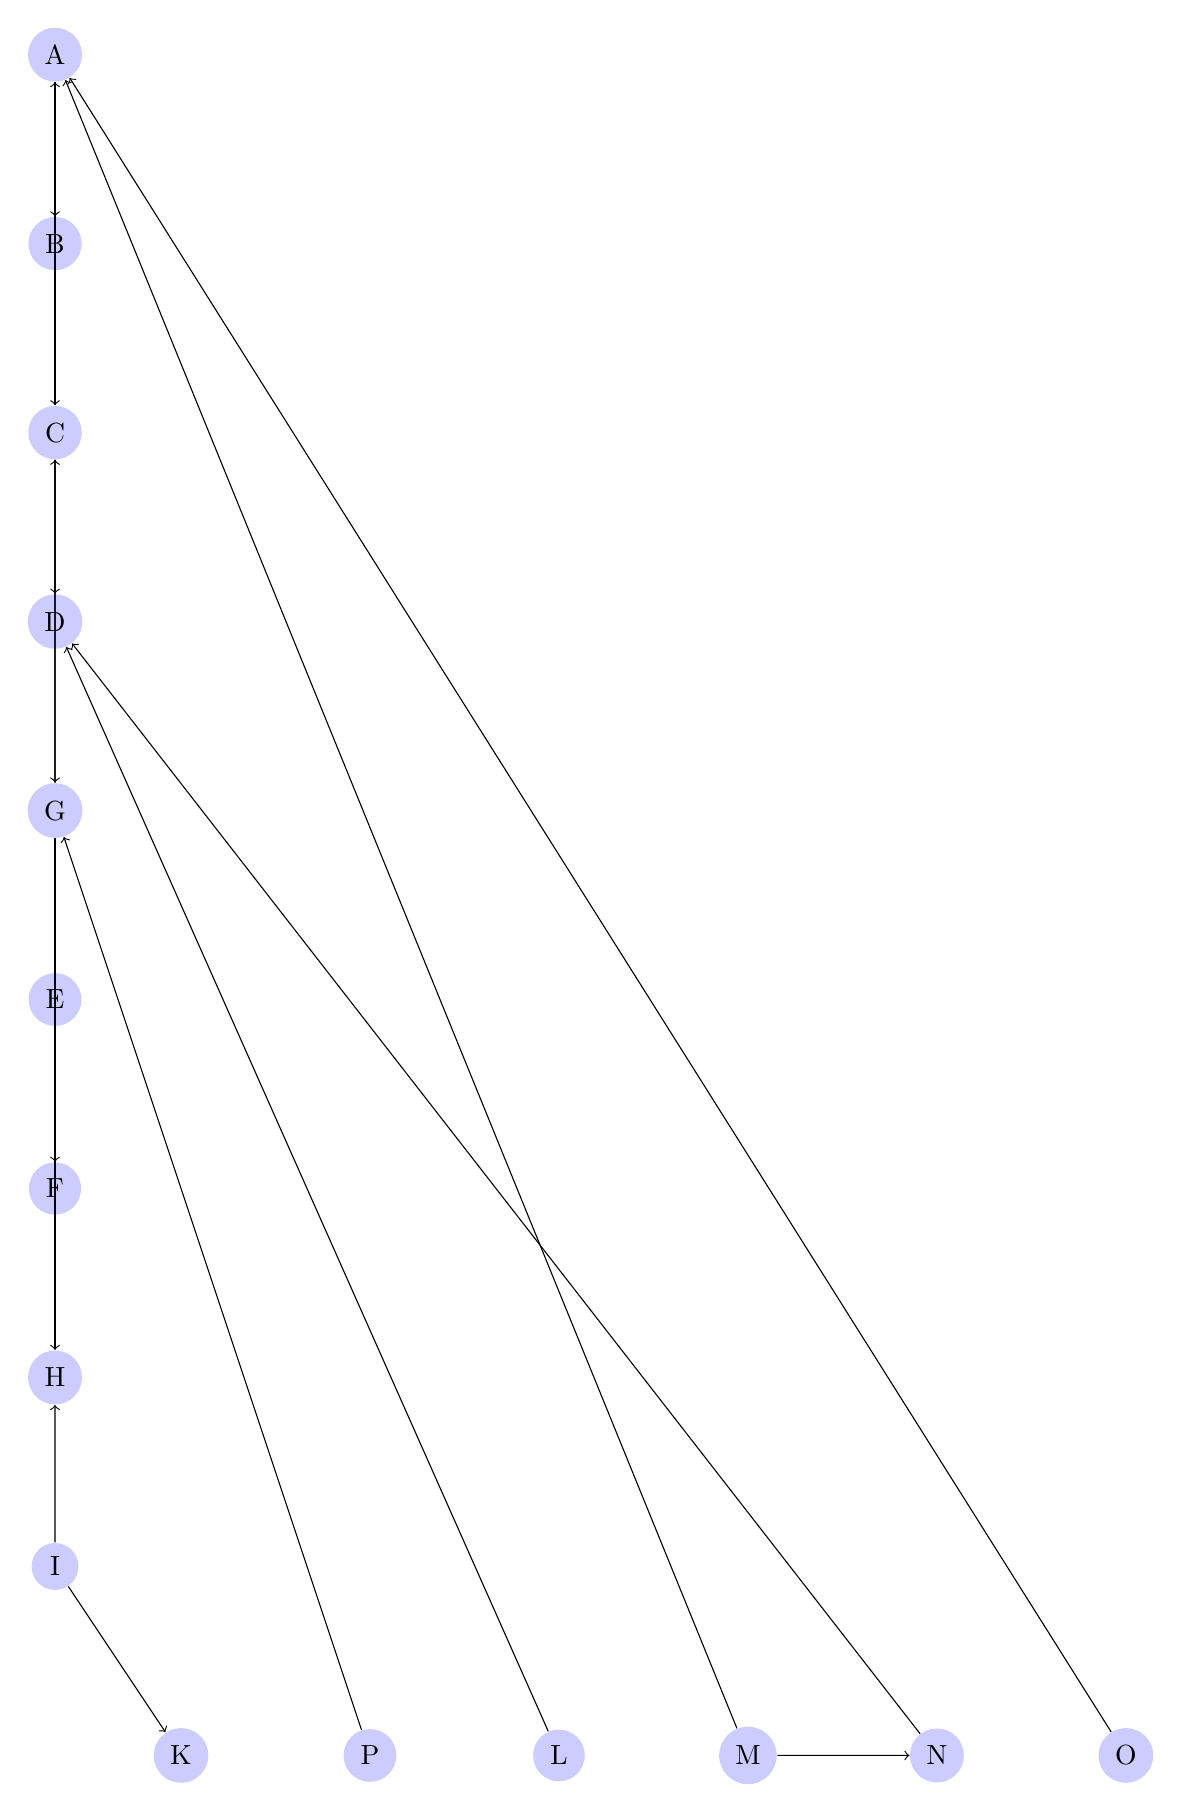
\begin{tikzpicture}[->,scale=.8,auto=left,every node/.style={circle,fill=blue!20}]
  \node (n1) at (3,1) {K};
  \node (n2) at (6,1)  {P};
  \node (n3) at (9,1)  {L};
  \node (n4) at (12,1) {M};
  \node (n5) at (15,1)  {N};
  \node (n6) at (18,1)  {O};
  \node (n7) at (1,4)  {I};
  \node (n8) at (1,7)  {H};
  \node (n9) at (1,10)  {F};
  \node (n10) at (1,13)  {E};
  \node (n11) at (1,16)  {G};
  \node (n12) at (1,19)  {D};
  \node (n13) at (1,22)  {C};
  \node (n14) at (1,25)  {B};
  \node (n15) at (1,28)  {A};

  \foreach \from/\to in {n15/n14,n14/n13,n13/n12,n13/n15,n13/n11,n10/n9,n11/n13,n11/n8,n7/n8,n7/n1,n3/n12,n4/n15,n4/n5,n5/n12,n6/n15,n2/n11}
    \draw (\from) -- (\to);

\end{tikzpicture}

\begin{verbatim}
IN: M , O , P
SCC: C , B , G , A
OUT:  D , H 
Tendrils: K , I , L
Tubes: N
Disconnected: E , F

\end{verbatim}
     
   
%}

\end{homeworkProblem}
\clearpage
\newpage

\bibliographystyle{plain}
\bibliography{A1bibFile}

\end{document}
